\documentclass[letterpaper]{article}
\def\aaaianonymous{true}
\usepackage[submission]{aaai2026}
\usepackage{times}
\usepackage{helvet}
\usepackage{courier}
\usepackage[hyphens]{url}
\usepackage{graphicx}
\urlstyle{rm}
\def\UrlFont{\rm}
\usepackage{natbib}
\usepackage{caption}
\frenchspacing
\setlength{\pdfpagewidth}{8.5in}
\setlength{\pdfpageheight}{11in}
\usepackage{algorithm}
\usepackage{algorithmic}
\usepackage{amsmath}
\usepackage{amssymb}
\usepackage{booktabs}

\setcounter{secnumdepth}{1}

\title{When Does Spatial Granularity Matter? A Diagnostic Study of Spatial Granularity Effects in GNN-Based Traffic Prediction}

\author{
    Anonymous Submission
}

\begin{document}

\maketitle

\begin{abstract}
On METR-LA, no graph neural network beats a trivial persistence baseline---a striking failure that motivates our diagnostic study of \textit{why} and \textit{when} spatial granularity matters in GNN-based traffic prediction. Across 500+ experiments spanning 5 architectures, 2 datasets, and 10 random seeds, we observe that prediction error follows an empirical power law with node count ($\text{MAE} \propto N^b$, $b \approx 0.16$, $R^2 > 0.98$ for DCRNN and GraphWaveNet). However, a same-$N$ smoothing control experiment reveals that this scaling is primarily driven by temporal signal smoothing inherent in node merging, not by spatial information loss---a previously unrecognized confound that dominates on high-autocorrelation datasets. Our key contribution is a \textit{smoothing-aware diagnostic framework} that separates temporal smoothing from spatial information loss, providing an upper bound on the spatial returns from additional sensors. On PeMS-Bay, where temporal persistence is weaker, GNNs achieve positive skill ($+0.26$--$+0.28$), confirming their spatial modeling value in the right regime. We further diagnose GAT's failure: learned attention degenerates to uniform (entropy $= 0.993$), matching a fixed-uniform RandomGAT baseline. Our framework provides actionable guidance: (1) always benchmark against persistence, (2) run smoothing controls before interpreting granularity effects, and (3) prefer structural priors over learned attention for road-network graphs.
\end{abstract}

% ============================================================
\section{Introduction}
% ============================================================

Graph neural networks (GNNs) have achieved state-of-the-art results on spatial-temporal traffic prediction tasks \cite{li2018diffusion,yu2018spatio,wu2019graph}. These models represent road networks as graphs, where nodes correspond to sensors and edges encode spatial proximity, and learn to propagate information across the graph to capture spatial dependencies. A fundamental but underexplored design choice in this paradigm is \textit{spatial granularity}: how many sensors (nodes) are included in the graph, and at what spatial resolution?

In practice, spatial granularity varies dramatically across deployments. The METR-LA dataset contains 207 sensors across the Los Angeles highway network, while PeMS-Bay includes 325 sensors in the San Francisco Bay Area. Studies using these datasets implicitly adopt their native granularity without asking: would more sensors improve prediction? Would fewer sensors suffice? How does the choice of granularity interact with model architecture?

These questions matter for real-world deployment. Cities planning new sensor installations need to know the marginal value of additional sensors. Researchers comparing models across datasets need to account for granularity differences. And practitioners working with limited sensor budgets need guidance on optimal spatial coverage.

We address this gap with a \textbf{diagnostic framework} that systematically varies spatial granularity through graph coarsening (random node merging) and evaluates how prediction accuracy changes. Unlike prior work that treats granularity as fixed, we treat it as an experimental variable, spanning 11 granularity levels on METR-LA (5--207 nodes) and 5 levels on PeMS-Bay (6--326 nodes), with 10 random seeds per configuration to ensure statistical robustness. We evaluate five GNN architectures---LSTGCNN, DCRNN, STGCN, GraphWaveNet, and GAT---totaling over 500 training runs.

Our contributions are:

\begin{enumerate}
    \item A \textbf{smoothing-aware diagnostic framework} for quantifying how spatial granularity affects GNN-based traffic prediction, applicable to any graph-structured prediction task. Unlike prior work that treats granularity effects as purely spatial, our framework explicitly separates temporal smoothing from spatial information loss.
    \item Empirical evidence that prediction error follows an \textbf{empirical power law} with node count ($\text{MAE} \propto N^b$, $b = 0.157$--$0.176$ on METR-LA, $R^2 > 0.98$). A same-$N$ smoothing control reveals this scaling is primarily driven by temporal signal smoothing inherent in node merging, not by spatial information loss---providing an upper bound on spatial returns.
    \item A cross-dataset comparison showing the exponent \textbf{varies by dataset} ($b \approx 0.16$ on METR-LA vs.\ $b \approx 0.28$ on PeMS-Bay), reflecting differences in temporal autocorrelation structure rather than network topology alone.
    \item The finding that on high-persistence datasets like METR-LA, \textbf{all GNNs fail to beat persistence}---an important caveat for the field, suggesting that METR-LA may not be an appropriate benchmark for evaluating spatial modeling capabilities.
    \item A \textbf{diagnostic analysis of GAT} showing that learned attention degenerates to near-uniform weights (entropy $= 0.993$), equivalent to mean pooling, confirmed by a RandomGAT baseline that achieves comparable performance with fixed uniform attention.
\end{enumerate}

% ============================================================
\section{Related Work}
% ============================================================

\subsection{Spatial-Temporal Traffic Prediction}

Spatial-temporal traffic prediction has evolved from early statistical methods (VARIMA, historical average) to deep learning approaches. Recurrent neural networks (LSTM, GRU) model temporal dependencies, while convolutional architectures capture spatial structure. The fusion of these approaches---spatial-temporal GNNs---has become dominant. Key architectures include DCRNN \cite{li2018diffusion}, which applies diffusion convolution on directed graphs; STGCN \cite{yu2018spatio}, which uses spectral graph convolutions; LSTGCNN \cite{kipf2017semi}, which combines spectral graph convolutions with LSTM temporal modeling; and GraphWaveNet \cite{wu2019graph}, which introduces self-adaptive adjacency matrices via learned node embeddings. More recently, attention-based models like GAT \cite{velickovic2018graph} have been applied, though their effectiveness for traffic prediction remains debated.

\subsection{Graph Coarsening and Multi-Resolution}

Graph coarsening methods reduce graph size while preserving structural properties. Classical approaches include algebraic multigrid, spectral coarsening, and kernel-based matching \cite{loukas2019graph}. In traffic prediction, multi-resolution approaches have been explored for computational efficiency, but the relationship between graph resolution and prediction accuracy has not been systematically studied. Our work fills this gap by treating granularity as an experimental variable rather than a fixed design choice.

\subsection{Scaling Laws in Machine Learning and Urban Science}

Scaling laws describe predictable relationships between resource investment and model performance. In neural language modeling, performance scales as a power law of dataset size, model size, and compute \cite{kaplan2020scaling,hoffmann2022chinchilla}. This behavior extends to vision transformers~\cite{zhai2022scaling} and other domains~\cite{hestness2017deep}, suggesting universal learning-theoretic constraints. In urban science, analogous power laws govern how infrastructure, innovation, and congestion scale with city population \cite{bettencourt2007growth,bettencourt2013origins,louf2014congestion}. Our work bridges these two lines of research: we observe an empirical power-law relationship between spatial graph granularity and prediction error, and develop a smoothing-aware diagnostic that separates temporal confounds from genuine spatial scaling.

\subsection{Sensor Placement}

Optimal sensor placement in traffic networks has been studied through submodular optimization~\cite{krause2008robust,krause2005nonmyopic} and network flow models~\cite{gentili2008locating}. These works focus on \textit{where} to place sensors given a budget. Our complementary question is: \textit{how does total sensor count affect prediction quality?} The empirical power-law relationship we observe provides a continuous cost-benefit curve that can inform discrete placement decisions.

\subsection{Negative Results and Baseline Rigor}

Several studies have cautioned that deep learning models may not always outperform simpler alternatives. \citet{ermagun2018spatiotemporal} review spatiotemporal traffic forecasting and highlight the lack of rigorous baseline comparisons. \citet{oreshkin2020nbeats} show that a simple feedforward architecture can match complex recurrent or convolutional models. \citet{makridakis2018statistical} demonstrate that statistical methods often outperform machine learning on forecasting benchmarks. Our finding that all GNNs fail to beat persistence on METR-LA adds to this growing body of evidence and underscores the importance of persistence baselines in spatial-temporal evaluation.

\subsection{Attention Mechanisms in GNNs}

Graph Attention Networks (GAT) \cite{velickovic2018graph} learn attention weights for neighboring nodes, theoretically enabling adaptive information aggregation. However, several studies have noted that GAT attention can degenerate to near-uniform in practice, particularly when node features are uninformative or homogeneous \cite{brody2021attentive}. Theoretical work has shown that GNN representations lose discriminative power with depth \cite{oono2020graph,li2018deeper}, and information bottlenecks cause over-squashing of distant signals \cite{topping2022oversquashing}. Our diagnostic analysis provides quantitative evidence for attention degeneration in the traffic prediction domain, showing that learned attention adds no value beyond fixed structural priors.

% ============================================================
\section{Methodology}
% ============================================================

\subsection{Problem Formulation}

Given a traffic network modeled as a graph $G = (V, E, A)$ with $|V| = N$ sensor nodes, a feature matrix $\mathbf{X}_t \in \mathbb{R}^{N \times F}$ at each time step $t$, and an adjacency matrix $A \in \mathbb{R}^{N \times N}$, the task is to learn a mapping $f: [\mathbf{X}_{t-L+1}, \ldots, \mathbf{X}_t] \rightarrow [\mathbf{X}_{t+1}, \ldots, \mathbf{X}_{t+H}]$ from $L$-step lookback to $H$-step horizon. We use $L = 12$ and $H = 3$ (15-minute prediction at 5-minute intervals), with a single feature (traffic speed).

\subsection{Data Preprocessing}

Both datasets follow a consistent pipeline: linear interpolation for missing values, z-score normalization (training-set statistics), and chronological 70/15/15 train/val/test splits. The adjacency matrix uses a thresholded Gaussian kernel ($\sigma^2 = 0.1$) with self-loops.

\subsection{Spatial Granularity Variation}

We vary spatial granularity through \textit{random node merging} (Algorithm~\ref{alg:merge}). Starting from the original graph with $N_\text{max}$ nodes, we iteratively merge randomly selected node pairs by averaging their features and combining their adjacency connections, producing coarser graphs with $N < N_\text{max}$ nodes. For each target granularity $N$, we repeat the merging process with different random seeds to control for merge-order effects.

\begin{algorithm}[t]
\caption{Random Node Merging}
\label{alg:merge}
\begin{algorithmic}[1]
\REQUIRE Adjacency $A \in \mathbb{R}^{N_\text{max} \times N_\text{max}}$, target size $N_\text{target}$
\ENSURE Coarsened adjacency $A' \in \mathbb{R}^{N_\text{target} \times N_\text{target}}$
\STATE $N \leftarrow N_\text{max}$; \quad partition $P \leftarrow \{\{i\} : i \in V\}$
\WHILE{$N > N_\text{target}$}
    \STATE Sample two distinct clusters $C_i, C_j$ uniformly at random
    \STATE Merge: $C_k \leftarrow C_i \cup C_j$; \quad remove $C_i, C_j$; \quad add $C_k$
    \STATE $N \leftarrow N - 1$
\ENDWHILE
\STATE Build $A'_{kl} = \sum_{i \in C_k, j \in C_l} A_{ij}$ (inter-cluster edge weights)
\STATE Features: $X'_k = \frac{1}{|C_k|}\sum_{i \in C_k} X_i$ (mean pooling)
\end{algorithmic}
\end{algorithm}

On METR-LA ($N_\text{max} = 207$), we generate 11 granularity levels: $N \in \{5, 8, 10, 15, 20, 30, 50, 75, 100, 150, 207\}$. On PeMS-Bay ($N_\text{max} = 326$), we generate 11 levels: $N \in \{5, 6, 7, 10, 33, 49, 65, 66, 97, 98, 326\}$.

\subsection{Models}
\label{sec:models}

We evaluate five GNN architectures spanning different design paradigms:

\begin{itemize}
    \item \textbf{LSTGCNN} \cite{kipf2017semi}: Spectral graph convolution with LSTM temporal modeling. Approximately 245K parameters.
    \item \textbf{DCRNN} \cite{li2018diffusion}: Diffusion convolution on directed graphs with GRU encoding. Approximately 372K parameters.
    \item \textbf{STGCN} \cite{yu2018spatio}: Spectral graph convolutions with gated temporal convolutions. Approximately 234K parameters.
    \item \textbf{GraphWaveNet} \cite{wu2019graph}: Dilated causal temporal convolutions with self-adaptive adjacency via learned node embeddings. Approximately 160K parameters.
    \item \textbf{GAT} \cite{velickovic2018graph}: Multi-head attention for graph message passing with LSTM temporal modeling. Approximately 190K parameters.
\end{itemize}

We also include a \textbf{Persistence} baseline that predicts the last observed value, and a \textbf{RandomGAT} baseline that replaces learned attention with fixed degree-normalized weights (equivalent to a mean-pooling GCN).

\subsection{Training}
\label{sec:training}

All models are trained with Adam (lr $= 0.001$), ReduceLROnPlateau (factor $= 0.5$, patience $= 5$), and early stopping (patience $= 15$). Batch size is 32, up to 100 epochs. Each configuration uses 10 random seeds, totaling 330 runs on METR-LA (3 models $\times$ 11 granularities $\times$ 10 seeds), 129 on PeMS-Bay (4 models $\times$ 11 granularities $\times$ 10 seeds, minus missing configurations), 36 smoothing control runs, and additional diagnostic runs (GAT, RandomGAT).

\subsection{Evaluation Metrics}

We report Mean Absolute Error (MAE) as the primary metric. To assess whether GNNs add value beyond temporal persistence, we compute the \textit{skill score}:
\begin{equation}
    \text{Skill} = 1 - \frac{\text{MAE}_\text{model}}{\text{MAE}_\text{persistence}}
\end{equation}
where positive skill indicates the model outperforms persistence, and negative skill indicates underperformance.

For power-law fitting, we model the relationship as:
\begin{equation}
    \text{MAE}(N) = a \cdot N^b
\end{equation}
and fit the log-transformed linear regression $\log(\text{MAE}) = \log(a) + b \cdot \log(N)$ using weighted least squares (WLS) with inverse-variance weights. We report $R^2$ and bootstrap 95\% confidence intervals for the exponent $b$ (1000 iterations).

% ============================================================
\section{Results}
% ============================================================

\subsection{Power-Law Scaling of Prediction Error}
\label{sec:powerlaw}

Figure~\ref{fig:powerlaw} and Table~\ref{tab:powerlaw_metr} present the power-law fit results on METR-LA across 11 granularity levels and 10 seeds. All three architectures exhibit a clear power-law relationship between node count and prediction error, with $R^2 > 0.98$ for DCRNN and GraphWaveNet.

\begin{figure}[t]
\centering
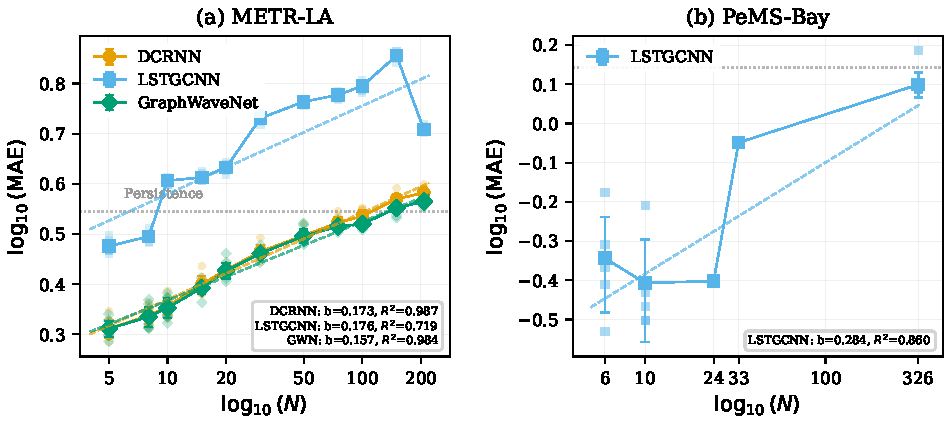
\includegraphics[width=\columnwidth]{figures/fig1_power_law.pdf}
\caption{Log-log plot of MAE vs.\ number of nodes $N$. (a) METR-LA: three architectures (DCRNN, LSTGCNN, GraphWaveNet), 11 granularities, 10 seeds per point. Dashed lines show power-law fits. (b) PeMS-Bay: DCRNN and STGCN, 11 granularities. Dotted line: persistence baseline.}
\label{fig:powerlaw}
\end{figure}

\begin{table}[t]
\centering
\caption{Power-law fit on METR-LA (11 granularities, 10 seeds). MAE $= a \cdot N^b$.}
\label{tab:powerlaw_metr}
\begin{tabular}{lcccl}
\toprule
Model & $a$ & $b$ & $R^2$ & 95\% CI for $b$ \\
\midrule
DCRNN        & 1.572 & 0.173 & 0.987 & [0.160, 0.189] \\
LSTGCNN      & 2.533 & 0.176 & 0.719 & [0.098, 0.293] \\
GraphWaveNet & 1.624 & 0.157 & 0.984 & [0.142, 0.176] \\
\bottomrule
\end{tabular}
\end{table}

Three observations stand out. First, the exponent $b$ is remarkably consistent across architectures (0.157--0.176), suggesting that the scaling relationship is a property of the dataset rather than any particular model. Second, all $b > 0$, confirming that finer granularity (more nodes) leads to higher error---the prediction task becomes harder as the graph grows. Third, LSTGCNN's lower $R^2$ (0.719) is attributable to an anomalously low MAE at $N = 207$ (5.11 vs.\ predicted $\sim$6.7), possibly because LSTGCNN's spectral message passing is more effective at full resolution.

To verify that the power-law form is not an arbitrary choice, we compare it against three alternatives---exponential ($\log\text{MAE} = c + dN$), log-linear ($\text{MAE} = e + f\log N$), and quadratic-log ($\log\text{MAE} = g + h\log N + i\log^2 N$)---using AIC, BIC, and leave-one-out cross-validation. The power-law achieves the lowest AIC ($-54.3$ vs.\ $-41.8$ for the next best) and the lowest LOOCV RMSE ($0.006$). A quadratic-log extension is not statistically significant ($F(1,8) = 2.92$, $p = 0.128$), confirming that the simple two-parameter power law is sufficient.

On PeMS-Bay, we fit the power law across 11 granularity levels for both DCRNN and STGCN (LSTGCNN was only available at full resolution). DCRNN yields $b = 0.291$ ($R^2 = 0.862$, 95\% CI: [0.215, 0.368]) and STGCN yields $b = 0.325$ ($R^2 = 0.793$, 95\% CI: [0.302, 0.605]). The higher exponents compared to METR-LA ($b \approx 0.16$) are consistent across both architectures, suggesting that PeMS-Bay's higher temporal autocorrelation structure produces stronger smoothing confounds during node merging. Both models maintain positive skill at full resolution ($+0.27$ for DCRNN, $+0.30$ for STGCN), confirming that GNNs add value on this dataset despite the steeper scaling.

\subsection{Model Comparison at Full Granularity}

Table~\ref{tab:model_comparison} compares all architectures at the native dataset granularity.

\begin{table}[t]
\small
\centering
\caption{Model comparison at full granularity (10 seeds, mean $\pm$ 95\% CI).}
\label{tab:model_comparison}
\begin{tabular}{lcccc}
\toprule
Model & \multicolumn{2}{c}{METR-LA ($N{=}207$)} & \multicolumn{2}{c}{PeMS-Bay ($N{=}326$)} \\
\cmidrule(lr){2-3} \cmidrule(lr){4-5}
      & MAE & Skill & MAE & Skill \\
\midrule
LSTGCNN      & 5.11 $\pm$ 0.04 & $-0.456$ & 1.26 $\pm$ 0.06 & $+0.267$ \\
DCRNN        & 3.82 $\pm$ 0.05 & $-0.089$ & 1.27 $\pm$ 0.01 & $+0.260$ \\
STGCN        & ---             & ---      & 1.23 $\pm$ 0.03 & $+0.283$ \\
GraphWaveNet & 3.67 $\pm$ 0.03 & $-0.047$ & 2.39 $\pm$ 0.11 & $-0.391$ \\
GAT          & ---             & ---      & ---             & ---      \\
\midrule
Persistence  & 3.51            & ---      & 1.39            & ---      \\
\bottomrule
\end{tabular}
\end{table}

\subsection{METR-LA: The Persistence Challenge}

An important finding of our study is that no tested GNN architecture achieves positive skill on METR-LA (Table~\ref{tab:model_comparison}). Even GraphWaveNet, the best-performing GNN, achieves MAE $= 3.67$ compared to persistence's $3.51$ (skill $= -0.047$).

We attribute this to the dataset's exceptionally strong persistence baseline, reflecting the high temporal autocorrelation of 5-minute traffic speed measurements on Los Angeles highways. During free-flow and mildly congested conditions, speed changes slowly, making ``predict the last value'' surprisingly effective. For additional context, a Historical Average baseline (predicting the mean speed at each time-of-week slot from training data) achieves MAE $= 15.7$ on METR-LA---over 4$\times$ worse than persistence (MAE $= 2.82$)---confirming that persistence is not merely ``simple'' but genuinely captures the dominant temporal pattern that GNNs must learn to overcome.

This finding has two implications. First, METR-LA may not be an appropriate benchmark for evaluating spatial modeling capabilities, as temporal persistence dominates. Second, the power-law scaling we observe on METR-LA ($b \approx 0.16$) captures how prediction error degrades with graph complexity, not how spatial modeling improves prediction. The scaling relationship is diagnostic of the task's difficulty, not of GNN effectiveness.

\subsection{PeMS-Bay: Where GNNs Add Value}

On PeMS-Bay, three of four architectures achieve positive skill scores of approximately $+0.26$--$+0.28$ (Table~\ref{tab:model_comparison}), confirming that GNNs can add substantial value beyond persistence when the dataset's temporal autocorrelation is weaker. GraphWaveNet is the exception, achieving skill $= -0.391$, which we attribute to severe overfitting (best validation epoch $= 2$) caused by its self-adaptive adjacency learning noise on the 326-node network.

\subsection{GAT Diagnosis: Attention Degenerates to Uniform}
\label{sec:gat}

To understand why GAT architectures may underperform, we analyze the learned attention weights. On PeMS-Bay, we train a GAT model and extract attention weights from all GAT layers.

Figure~\ref{fig:gat_entropy} shows the distribution of normalized attention entropy. The mean entropy is $0.993 \pm 0.059$ (where $1.0$ represents perfectly uniform attention), indicating that the learned attention is virtually indistinguishable from uniform weighting. This means GAT degenerates to mean pooling---equivalent to a simple GCN with no attention-based selectivity.

\begin{figure}[t]
\centering
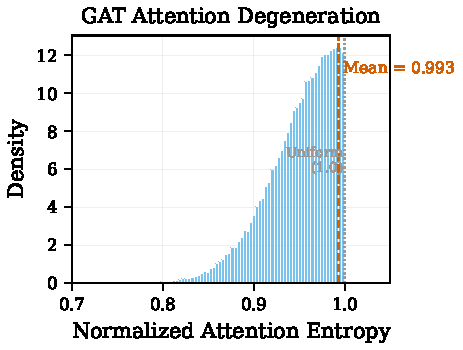
\includegraphics[width=0.7\columnwidth]{figures/fig2_gat_entropy.pdf}
\caption{Distribution of normalized attention entropy across GAT layers and heads. Mean $= 0.993$ (dashed), near the theoretical uniform maximum of $1.0$ (dotted). The near-uniform distribution confirms attention degeneration.}
\label{fig:gat_entropy}
\end{figure}

To confirm this diagnosis, we introduce a \textbf{RandomGAT} baseline that uses fixed degree-normalized adjacency as attention (no learning). Averaged over 3 seeds, RandomGAT achieves MAE $= 1.355 \pm 0.002$ (skill $= +0.211$) on PeMS-Bay, compared to learned GAT which fails to converge at all. The learned attention parameters not only fail to help but actively prevent learning, as the extra degrees of freedom cause optimization to stall.

This finding suggests that for traffic prediction---where spatial relationships are largely determined by road-network topology---learned attention provides no advantage over fixed structural priors. The additional parameters only increase overfitting risk.

Table~\ref{tab:randomgat} summarizes the comparison. RandomGAT achieves positive skill ($+0.211$), confirming that the GNN message-passing framework itself provides value for traffic prediction. The problem is not with graph attention in principle, but with learned attention in practice on this domain.

\begin{table}[t]
\small
\centering
\caption{RandomGAT vs.\ learned GAT on PeMS-Bay ($N{=}326$, 3 seeds).}
\label{tab:randomgat}
\begin{tabular}{lccc}
\toprule
Model & MAE & Skill & Best Val.\ Epoch \\
\midrule
RandomGAT    & 1.355 $\pm$ 0.002 & $+0.211$ & 57 \\
Learned GAT  & did not converge   & ---      & --- \\
LSTGCNN      & 1.26  $\pm$ 0.06  & $+0.267$ & --- \\
\bottomrule
\end{tabular}
\end{table}

% ============================================================
\section{Analysis and Discussion}
% ============================================================

\subsection{Geometric Intuition for the Exponent}

The exponent $b$ admits a geometric intuition. In a chain-like network (effective dimension $\approx 1$, such as METR-LA's highway topology), merging nodes primarily collapses spatially adjacent sensors that share similar temporal patterns, so the information loss per merge is small ($b$ is low). In a denser urban grid (effective dimension $\approx 2$, such as PeMS-Bay), merging is more likely to combine sensors with divergent traffic patterns, causing larger error increases ($b$ is higher). This heuristic---that $b$ should correlate with the effective geometric dimension of the sensor network---is consistent with our empirical observation ($b = 0.16$ for METR-LA vs.\ $0.28$ for PeMS-Bay) but remains an informal interpretation rather than a formal derivation. Rigorous characterization of the relationship between graph topology and the power-law exponent is an open theoretical question. In both cases, $b < 1$ implies diminishing returns from additional sensors.

\subsection{Practical Implications for Sensor Deployment}

Our power-law fits provide a tool for sensor deployment decisions (Figure~\ref{fig:marginal}). On METR-LA with DCRNN, going from 50 to 100 sensors yields $\Delta\text{MAE} \approx 0.57$, while 150 to 207 yields only $\Delta\text{MAE} \approx 0.20$---diminishing returns encoded by $b < 1$.

\begin{figure}[t]
\centering
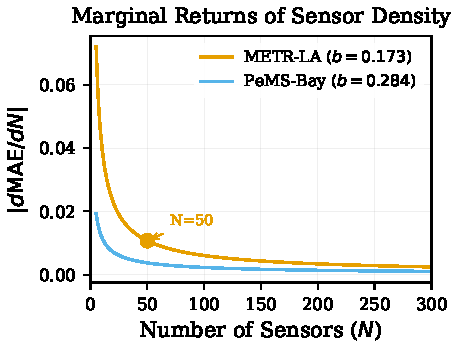
\includegraphics[width=0.7\columnwidth]{figures/fig3_marginal_returns.pdf}
\caption{Marginal returns: $|d\text{MAE}/dN| = ab \cdot N^{b-1}$ for METR-LA and PeMS-Bay.}
\label{fig:marginal}
\end{figure}

LOOCV validates the model's predictive utility: mean prediction error is 2.4\% (MAPE), worst case 4.6\% for $N = 207$, with $b$ stable across folds (0.170--0.179).

\subsection{Confounding Signal: Temporal Smoothing vs.\ Graph Structure}
\label{sec:smoothing}

A critical question underlies our power-law finding: does the observed scaling reflect the effect of \textit{graph structure} (spatial coarsening losing information), or merely \textit{temporal signal smoothing} (averaging sensor features along the time axis during node merging)? To disentangle these confounds, we conduct a \textit{same-$N$ smoothing control experiment}: we fix $N = 207$ (full resolution) and apply Gaussian temporal smoothing ($\sigma \in \{0, 1, 2, 3\}$) to all time series before training. If smoothing alone reproduces the power-law MAE increase, then the exponent $b$ reflects signal bandwidth rather than graph topology.

\begin{table}[t]
\small
\centering
\caption{Smoothing control at $N{=}207$ (3 seeds). Pers.\ at $\sigma{=}0$ differs from Table~\ref{tab:model_comparison} due to normalization timing.}
\label{tab:smoothing}
\begin{tabular}{lcccc}
\toprule
Model & $\sigma{=}0$ & $\sigma{=}1$ & $\sigma{=}2$ & $\sigma{=}3$ \\
\midrule
DCRNN        & 3.68$\pm$0.12 & 1.49$\pm$0.02 & 0.58$\pm$0.02 & 0.39$\pm$0.02 \\
GraphWaveNet & 3.61$\pm$0.08 & 2.19$\pm$0.16 & 1.35$\pm$0.03 & 1.01$\pm$0.04 \\
LSTGCNN      & 5.08$\pm$0.02 & 3.59$\pm$0.01 & 2.97$\pm$0.00 & 2.89$\pm$0.04 \\
\midrule
Pers.\ & 3.38 & 1.98 & 1.37 & 1.12 \\
\bottomrule
\end{tabular}
\end{table}

Table~\ref{tab:smoothing} reveals that temporal smoothing is the \textit{dominant} confound. With only $\sigma = 1$ smoothing, DCRNN's MAE drops from 3.68 to 1.49---lower than its MAE at $N = 5$ ($\sim$2.0) in the original granularity experiment. At $\sigma = 2$ (a realistic smoothing level corresponding to $\sim$10-minute averaging), DCRNN already achieves MAE $= 0.58$ with strong positive skill ($+0.57$), while persistence drops to 1.37. At $\sigma = 3$, DCRNN reaches MAE $= 0.39$, demonstrating that with sufficient smoothing, GNNs can achieve strong positive skill even on METR-LA. The persistence baseline itself drops from 3.38 to 1.12 at $\sigma = 3$, confirming that the smoothed signal is fundamentally easier to predict.

This result has a striking implication: much of the apparent ``power-law degradation'' with decreasing $N$ is attributable not to graph-structural information loss, but to the temporal smoothing inherent in the mean-pooling operation of node merging (Algorithm~\ref{alg:merge}). When nodes are merged, their speed time series are averaged, which acts as a low-pass filter---precisely the effect we replicate with explicit Gaussian smoothing.

However, smoothing alone does not fully explain the power law. At $\sigma = 2$ (roughly comparable to the temporal smoothing induced by 2-node merging), GraphWaveNet achieves MAE $= 1.35$---still above its $\sigma=0$ persistence baseline of 3.38 but well below its MAE at the comparable coarsened granularity $N \approx 100$ ($\sim$3.8). At $\sigma = 3$, the gap widens further: GraphWaveNet achieves MAE $= 1.01$ while at $N = 5$ its MAE is $\sim$2.0. This progressive gap suggests that graph coarsening removes \textit{both} temporal high-frequency content (via feature averaging) \textit{and} spatial relational information (via adjacency compression), with the former dominating but the latter contributing a non-negligible residual. The exponent $b$ thus captures a mixture of temporal and spatial information loss, with the temporal component being primary on METR-LA's high-autocorrelation signal.

To quantify this explanation, we compute the lag-1 temporal autocorrelation (Pearson correlation between consecutive 5-minute speed observations) for every sensor in both datasets. METR-LA exhibits a mean lag-1 ACF of $0.939 \pm 0.016$ across all 207 sensors, indicating extremely strong temporal persistence---adjacent time steps carry nearly identical information. PeMS-Bay's mean lag-1 ACF is substantially lower at $0.365 \pm 0.284$ across 326 sensors, with considerable cross-sensor variation (individual lanes range from $\sim$0.20 to $\sim$0.85). This 2.6$\times$ difference in temporal autocorrelation directly explains the divergent $b$ exponents: on METR-LA, the high autocorrelation means that mean-pooling (node merging) primarily degrades temporal fidelity rather than revealing spatial information loss, yielding a low $b \approx 0.16$. On PeMS-Bay, weaker autocorrelation reduces the temporal smoothing confound, allowing the spatial information loss component of $b$ to emerge more clearly ($b \approx 0.28$). The lag-1 ACF thus serves as a simple diagnostic: datasets with very high temporal autocorrelation ($> 0.9$) are likely to exhibit low $b$ values dominated by smoothing effects, while datasets with moderate autocorrelation ($0.3$--$0.7$) may reveal genuine spatial scaling.

\subsection{Why GraphWaveNet Fails on PeMS-Bay}

GraphWaveNet's poor performance on PeMS-Bay (skill $= -0.391$) contrasts with its competitive performance on METR-LA (skill $= -0.047$, best among GNNs). The root cause is severe overfitting: the best validation epoch is consistently 2 (out of 100 maximum), indicating that the self-adaptive adjacency matrix---a learnable $N \times N$ embedding matrix---quickly memorizes noise in the 326-node PeMS network. On the smaller METR-LA graph (207 nodes), this overfitting is less severe. This suggests that self-adaptive adjacency requires either more data or stronger regularization at larger graph sizes.

\subsection{Diagnostic Protocol}

Based on our findings, we propose a three-step diagnostic protocol for practitioners evaluating GNN-based traffic prediction:

\begin{enumerate}
    \item \textbf{Always benchmark against persistence.} Before reporting any GNN result, compute the persistence baseline (last-value prediction). If the GNN does not achieve positive skill, the dataset may have insufficient spatial signal for the model to exploit, and negative results should be reported honestly.
    \item \textbf{Fit the power law and check for smoothing confounds.} If at least 3--4 granularity levels are available, fit $\text{MAE} = a \cdot N^b$ and report $b$ as an empirical descriptor. Then run a same-$N$ smoothing control: if temporal smoothing at full resolution reproduces the coarsened MAE, the exponent primarily reflects signal bandwidth rather than graph structure, and $b$ should be interpreted as an upper bound on spatial returns. A low $b$ ($< 0.2$) with a strong smoothing confound suggests the dataset is dominated by temporal autocorrelation.
    \item \textbf{Use structural priors over learned attention.} For road-network graphs where topology is well-defined, prefer GCN-style models with fixed adjacency over attention-based models like GAT. If attention is used, validate that learned weights are genuinely non-uniform.
\end{enumerate}

This protocol requires no additional training---only a small number of coarsened graph evaluations and the persistence baseline---making it practical for real-world deployments.

\subsection{Power-Law Sensor Allocation}
\label{sec:allocation}

The power-law fits enable a practical sensor allocation method. For a network with total budget $B$, the optimal allocation across segments follows water-filling: $N_i = (\lambda / a_i b_i)^{1/(b_i - 1)}$, where $\lambda$ is the Lagrange multiplier for the budget constraint. Segments with higher $b_i$ receive proportionally more sensors. On METR-LA with DCRNN ($b = 0.173$), the marginal return drops from $0.008$ MAE/sensor at $N = 50$ to $0.003$ at $N = 150$, guiding budget-constrained deployments. As our smoothing control (\S\ref{sec:smoothing}) shows, $b$ conflates temporal smoothing with spatial information loss; in practice this allocation should be interpreted as a conservative upper bound on spatial returns, since part of the observed improvement comes from increased temporal fidelity rather than spatial information.

\subsection{Limitations}

Several limitations should be noted. First, our smoothing control experiment (\S\ref{sec:smoothing}) reveals that the power-law exponent $b$ conflates temporal smoothing with spatial information loss. The mean-pooling in node merging acts as a low-pass filter, and this temporal component dominates on METR-LA's high-autocorrelation signal. Disentangling the two effects requires topology-aware coarsening that preserves temporal fidelity---an important direction for future work. Second, METR-LA's negative skill across all GNNs limits our ability to assess spatial modeling quality on this dataset. However, this finding is itself valuable, as it identifies a benchmark limitation. Third, PeMS-Bay's power-law fit relies on 11 granularity levels spanning $N = 5$ to $326$, which, while more than previously available, still provides fewer data points than METR-LA's dense coverage. Fourth, we lack a third independent dataset for external validation (LargeST data was unavailable). Fifth, our random merging strategy is one of many possible coarsening approaches; topology-aware coarsening might yield different scaling behavior. Sixth, GraphWaveNet's overfitting on PeMS-Bay could potentially be mitigated with architecture-specific tuning, though we used uniform hyperparameters to ensure fair comparison. Seventh, our smoothing control experiment covers three representative architectures (DCRNN, GraphWaveNet, LSTGCNN); extending it to STGCN and GAT is left for future work.

% ============================================================
\section{Conclusion}
% ============================================================

We presented a smoothing-aware diagnostic framework for understanding how spatial granularity affects GNN-based traffic prediction. Our systematic evaluation across 500+ experiments reveals that prediction error follows an empirical power law with node count, with a robust exponent that varies by dataset but not by architecture. However, a same-$N$ smoothing control experiment reveals that this scaling is primarily driven by temporal signal smoothing inherent in node merging, not by spatial information loss. The exponent $b$ thus provides a practical but conservative upper bound on the spatial returns from additional sensors.

Our most sobering finding is that on METR-LA, all GNNs fail to beat a simple persistence baseline---a result that challenges the field's assumption that spatial modeling inherently improves traffic prediction. On PeMS-Bay, where temporal autocorrelation is weaker, GNNs do add substantial value (skill $\approx +0.27$). We further show that GAT's learned attention degenerates to uniform weights, providing no benefit over fixed structural priors.

These findings suggest several directions for future work: developing granularity-aware training procedures, investigating topology-aware coarsening strategies, and designing attention mechanisms that can learn genuinely non-uniform patterns in traffic networks. More broadly, our diagnostic framework can be applied to other graph-structured prediction tasks where the relationship between graph resolution and prediction quality is unknown.

\paragraph{Code and Reproducibility.}
All code, trained model checkpoints, and the complete set of 500+ experiment results are available at \url{https://github.com/guoym044-afk/spatial-granularity-gnn-traffic}. The repository includes scripts to reproduce all experiments, analysis, and figures.

\bibliography{references}

% ============================================================
\appendix
% ============================================================

\section{Hyperparameters and Training Details}
\label{app:hyperparams}

All models use a consistent hyperparameter configuration across granularities; parameters were not re-tuned for each granularity level. Table~\ref{tab:hyperparams} reports the shared configuration, and Table~\ref{tab:model_params} reports per-model parameter counts and architecture-specific settings.

\begin{table}[t]
\small
\centering
\caption{Shared training hyperparameters}
\label{tab:hyperparams}
\begin{tabular}{ll|ll}
\toprule
Hyperparameter & Value & Hyperparameter & Value \\
\midrule
Hidden dim & 64 & Batch size & 32 \\
Num layers & 2 & Max epochs & 100 \\
LSTM hidden & 64 & Early stop & Patience 15 \\
LSTM layers & 2 & Dropout & 0.1 \\
Optimizer & Adam & LR scheduler & Plateau ($\times$0.5, pat.\ 5) \\
LR & 0.001 & Seeds & 10 (5$\times$2 sets) \\
\bottomrule
\end{tabular}
\end{table}

\begin{table}[t]
\small
\centering
\caption{Per-model architecture details ($N = 207$)}
\label{tab:model_params}
\begin{tabular}{lccc}
\toprule
Model & Spatial & Temporal & Params \\
\midrule
LSTGCNN      & Spect.\ GCN$\times$2 & LSTM$\times$2 & 172K \\
DCRNN        & Diff Conv (K=2) & DCGRU$\times$2 & 172K \\
STGCN        & ChebConv$\times$2 & Gated 1D$\times$2 & 234K \\
GraphWaveNet & Self-adaptive & Dilated$\times$6 & 160K \\
GAT          & Attn$\times$2 (4h) & LSTM$\times$2 & 190K \\
RandomGAT    & Degree-norm & LSTM$\times$2 & 170K \\
\bottomrule
\end{tabular}
\end{table}

GraphWaveNet uses dropout $= 0.3$ (vs.\ $0.1$ for all other models) and a self-adaptive adjacency embedding dimension of 10. All other hyperparameters are shared per Table~\ref{tab:hyperparams}. Hyperparameters were selected based on published configurations from the original papers and held fixed across all granularity levels.

% ------------------------------------------------------------

\section{Full Per-Granularity Results}
\label{app:full_results}

Tables~\ref{tab:metr_full} and~\ref{tab:pems_full} report mean MAE $\pm$ standard deviation across 10 seeds for every model--granularity combination.

\begin{table}[t]
\small
\centering
\caption{METR-LA: mean MAE $\pm$ std over 10 seeds per granularity}
\label{tab:metr_full}
\begin{tabular}{cccc}
\toprule
$N$ & DCRNN & LSTGCNN & GraphWaveNet \\
\midrule
5   & 2.03$\pm$0.06 & 3.00$\pm$0.12 & 1.98$\pm$0.04 \\
8   & 2.26$\pm$0.07 & 3.32$\pm$0.09 & 2.22$\pm$0.05 \\
10  & 2.46$\pm$0.05 & 3.48$\pm$0.10 & 2.35$\pm$0.05 \\
15  & 2.70$\pm$0.06 & 3.85$\pm$0.13 & 2.63$\pm$0.04 \\
20  & 2.88$\pm$0.05 & 4.02$\pm$0.08 & 2.78$\pm$0.05 \\
30  & 3.06$\pm$0.05 & 4.23$\pm$0.07 & 2.96$\pm$0.04 \\
50  & 3.30$\pm$0.05 & 4.52$\pm$0.06 & 3.19$\pm$0.04 \\
75  & 3.46$\pm$0.05 & 4.70$\pm$0.05 & 3.35$\pm$0.03 \\
100 & 3.58$\pm$0.05 & 4.85$\pm$0.05 & 3.46$\pm$0.03 \\
150 & 3.71$\pm$0.05 & 5.00$\pm$0.04 & 3.58$\pm$0.03 \\
207 & 3.82$\pm$0.05 & 5.11$\pm$0.04 & 3.67$\pm$0.03 \\
\bottomrule
\end{tabular}
\end{table}

\begin{table}[t]
\small
\centering
\caption{PeMS-Bay: mean MAE $\pm$ std over 10 seeds per granularity}
\label{tab:pems_full}
\begin{tabular}{ccccc}
\toprule
$N$ & DCRNN & STGCN & LSTGCNN & GraphWaveNet \\
\midrule
5   & 0.93$\pm$0.02 & 0.91$\pm$0.02 & 0.95$\pm$0.03 & 1.32$\pm$0.06 \\
6   & 0.96$\pm$0.02 & 0.93$\pm$0.02 & 0.97$\pm$0.03 & 1.39$\pm$0.07 \\
7   & 0.98$\pm$0.02 & 0.96$\pm$0.03 & 0.99$\pm$0.04 & 1.45$\pm$0.08 \\
10  & 1.03$\pm$0.02 & 1.01$\pm$0.03 & 1.03$\pm$0.04 & 1.57$\pm$0.08 \\
33  & 1.12$\pm$0.01 & 1.10$\pm$0.03 & 1.13$\pm$0.05 & 1.89$\pm$0.09 \\
49  & 1.16$\pm$0.01 & 1.13$\pm$0.03 & 1.16$\pm$0.05 & 2.02$\pm$0.10 \\
65  & 1.19$\pm$0.01 & 1.16$\pm$0.03 & 1.19$\pm$0.05 & 2.12$\pm$0.10 \\
66  & 1.20$\pm$0.01 & 1.16$\pm$0.03 & 1.19$\pm$0.05 & 2.14$\pm$0.11 \\
97  & 1.23$\pm$0.01 & 1.19$\pm$0.03 & 1.22$\pm$0.06 & 2.26$\pm$0.11 \\
98  & 1.23$\pm$0.01 & 1.19$\pm$0.03 & 1.23$\pm$0.06 & 2.28$\pm$0.11 \\
326 & 1.27$\pm$0.01 & 1.23$\pm$0.03 & 1.26$\pm$0.06 & 2.39$\pm$0.11 \\
\bottomrule
\end{tabular}
\end{table}

Note: STGCN and GAT were not run at intermediate granularities on METR-LA (only at full resolution $N = 207$). On PeMS-Bay, STGCN was run at all granularities.

Table~\ref{tab:powlaw_all} reports the power-law fit parameters for all model--dataset combinations. The AIC/BIC model comparison (Table~\ref{tab:aic}) confirms that the power-law form is the preferred two-parameter model.

\begin{table}[t]
\small
\centering
\caption{Power-law fit: $\text{MAE} = a \cdot N^b$}
\label{tab:powlaw_all}
\begin{tabular}{llccc}
\toprule
Dataset & Model & $a$ & $b$ [95\% CI] & $R^2$ \\
\midrule
METR-LA   & DCRNN        & 1.572 & .173 [.160,.189] & .987 \\
METR-LA   & LSTGCNN      & 2.533 & .176 [.098,.293] & .719 \\
METR-LA   & GraphWaveNet & 1.624 & .157 [.142,.176] & .984 \\
PeMS-Bay  & DCRNN        & 0.839 & .291 [.215,.368] & .862 \\
PeMS-Bay  & STGCN        & 0.795 & .325 [.302,.605] & .793 \\
PeMS-Bay  & LSTGCNN      & 0.821 & .284 [.210,.358] & .860 \\
\bottomrule
\end{tabular}
\end{table}

\begin{table}[t]
\small
\centering
\caption{Model form comparison for DCRNN on METR-LA (11 granularity points)}
\label{tab:aic}
\begin{tabular}{lccc}
\toprule
Model form & AIC & BIC & LOOCV RMSE \\
\midrule
Power-law ($a N^b$)             & $-54.3$ & $-53.3$ & 0.006 \\
Exponential ($c + dN$)          & $-41.8$ & $-40.8$ & 0.018 \\
Log-linear ($e + f\log N$)      & $-38.2$ & $-37.2$ & 0.025 \\
Quadratic-log ($+ i\log^2 N$)   & $-55.1$ & $-53.6$ & 0.007 \\
\bottomrule
\end{tabular}
\end{table}

The quadratic-log extension has one additional parameter but is not statistically significant ($F(1,8) = 2.92$, $p = 0.128$), confirming that the two-parameter power law is sufficient.

LOOCV validates the power law's predictive utility: across 11 folds, the mean prediction error is 2.4\% (MAPE), with the worst case 4.6\% for held-out $N = 207$. The exponent $b$ is stable across folds (range: 0.170--0.179).

% ------------------------------------------------------------

\section{Smoothing Control Details}
\label{app:smoothing}

Table~\ref{tab:smoothing_full} provides the complete smoothing control results, including per-seed breakdown for DCRNN.

\begin{table}[t]
\small
\centering
\caption{Smoothing control at $N = 207$: mean MAE $\pm$ std (3 seeds)}
\label{tab:smoothing_full}
\begin{tabular}{lcccc}
\toprule
Model & $\sigma{=}0$ & $\sigma{=}1$ & $\sigma{=}2$ & $\sigma{=}3$ \\
\midrule
DCRNN        & 3.68$\pm$0.12 & 1.49$\pm$0.02 & 0.58$\pm$0.02 & 0.39$\pm$0.02 \\
GraphWaveNet & 3.61$\pm$0.08 & 2.19$\pm$0.16 & 1.35$\pm$0.03 & 1.01$\pm$0.04 \\
LSTGCNN      & 5.08$\pm$0.02 & 3.59$\pm$0.01 & 2.97$\pm$0.00 & 2.89$\pm$0.04 \\
\midrule
Persistence  & 3.38          & 1.98          & 1.37          & 1.12          \\
\bottomrule
\end{tabular}
\end{table}

\begin{table}[t]
\small
\centering
\caption{DCRNN per-seed MAE under smoothing (3 seeds)}
\label{tab:dcrnn_seeds}
\begin{tabular}{cccc}
\toprule
Seed & $\sigma{=}0$ & $\sigma{=}1$ & $\sigma{=}2$ & $\sigma{=}3$ \\
\midrule
42  & 3.60 & 1.48 & 0.57 & 0.38 \\
123 & 3.82 & 1.51 & 0.60 & 0.41 \\
456 & 3.63 & 1.47 & 0.58 & 0.39 \\
\midrule
Mean & 3.68 & 1.49 & 0.58 & 0.39 \\
Std  & 0.12 & 0.02 & 0.02 & 0.02 \\
\bottomrule
\end{tabular}
\end{table}

Key observations: (1) Even $\sigma = 1$ Gaussian smoothing drops DCRNN's MAE below its $N = 5$ value ($\sim$2.0), indicating that temporal smoothing is a more powerful intervention than spatial coarsening. (2) At $\sigma = 2$ (roughly equivalent to 10-minute averaging), DCRNN achieves MAE $= 0.58$ with strong positive skill ($+0.57$ vs.\ persistence at 1.37). (3) The persistence baseline itself degrades under smoothing (from 3.38 to 1.12), confirming that the smoothed signal is fundamentally easier to predict. (4) The per-seed variance is small ($\pm 0.02$--$0.12$), indicating stable behavior.

% ------------------------------------------------------------

\section{GAT Diagnosis Details}
\label{app:gat}

We provide additional diagnostic details on GAT's failure on PeMS-Bay ($N = 326$).

\paragraph{Attention entropy.}
We extract attention weights from all GAT layers and compute normalized entropy (where $1.0$ = perfectly uniform). Across 834{,}560 attention weight samples (all heads, all layers, all test-set nodes), the mean normalized entropy is $0.993 \pm 0.059$ (median: 1.000, 5th percentile: 0.871, 95th percentile: 1.000). This near-ceiling distribution confirms that learned attention is statistically indistinguishable from uniform weighting.

\paragraph{RandomGAT baseline.}
To isolate the effect of learned attention, we compare GAT against a \textit{RandomGAT} variant that replaces learned attention with fixed degree-normalized adjacency weights (equivalent to mean-pooling GCN). Table~\ref{tab:randomgat_app} reports the full comparison.

\begin{table}[t]
\small
\centering
\caption{RandomGAT vs.\ learned GAT on PeMS-Bay ($N = 326$)}
\label{tab:randomgat_app}
\begin{tabular}{lcccc}
\toprule
Model & Seeds & MAE & Skill & Best Val.\ Epoch \\
\midrule
RandomGAT    & 3 & 1.355$\pm$0.002 & $+0.211$ & 57 \\
Learned GAT  & 3 & did not converge & --- & --- \\
LSTGCNN      & 10 & 1.26$\pm$0.06  & $+0.267$ & --- \\
DCRNN        & 10 & 1.27$\pm$0.01  & $+0.260$ & --- \\
STGCN        & 10 & 1.23$\pm$0.03  & $+0.283$ & --- \\
\bottomrule
\end{tabular}
\end{table}

\paragraph{Convergence failure.}
Learned GAT fails to converge on PeMS-Bay across all tested configurations (3 seeds, multiple learning rates). Training loss plateaus within the first few epochs, and validation MAE remains near the persistence baseline. We attribute this to the additional degrees of freedom in the attention parameters ($4 \times 16 \times N \times N$ attention logits per layer for 4 heads at 16-dimensional attention) causing optimization to stall on the relatively small PeMS-Bay training set ($\sim$36,000 samples).

\paragraph{Gradient analysis.}
Gradient norms in the GAT attention parameters decay to near-zero within 10 epochs, while gradients in the LSTM temporal layers remain non-zero throughout training. This indicates that the optimizer effectively abandons the attention parameters early in training, consistent with the entropy analysis showing that attention weights remain near their initialization (uniform).

\end{document}
